\section{Approximate Abstraction on Example Domains}
%Explanation of what abstraction is used
We ran experiments on aggregation functions in the $\epQ$ family of approximate abstractions. We provide results for only $\epQ$ because, as our proofs in Section \ref{sec:theory_results} demonstrate, the other three functions are reducible to particular $\epQ$ functions. For the purpose of illustrating what kinds of approximations are possible, we built each abstraction by first solving the MDP, then greedily aggregating ground states into abstract states that satisfied the $\epQ$ criteria. Since this approach represents an order-dependent approximation to the maximum amount of abstraction possible, we randomized the order in which states were considered across trials. Every ground state is equally weighted in its abstract state.

%Explanation of what plots done
For each domain, we report two quantities as a function of epsilon with 95\% confidence bars. First, we compare the number of states in the abstract \ac{MDP} for different values of $\varepsilon$, shown in the top row of Figure~\ref{fig:main_empirical_results1}. The smaller the number of abstract states, the smaller the state space of the $\ac{MDP}$ that the agent must plan over. Second, we report the value under the abstract policy of the initial ground state, also shown in the bottom row of Figure~\ref{fig:main_empirical_results1} so the tradeoff between abstract state space size and near optimality is made evident. In the Taxi and Random domains, 200 trials were run for each data point, whereas 20 trials were sufficient for data points in Minefield and NChain.

%Discuss results
Our empirical results corroborate our thesis---approximate state abstractions can decrease state space size while retaining bounded error. In both NChain and Minefield, we observe that, as $\varepsilon$ increases from $0$, the number of states that must be planned over is reduced, and optimal behavior is either fully maintained (NChain) or very nearly maintained (Minefield). Similarly for Taxi, when $\varepsilon$ is between $.02$ and $.025$, we observe a reduction in the number of states in the abstract \ac{MDP} while value is fully maintained. After $.025$, increased reduction in state space size comes at a cost of value. Lastly, as $\varepsilon$ is increased in the Random domain, there is a smooth reduction in the number of abstract states with a corresponding cost in the value of the derived policy. When $\varepsilon = 0$, there is no reduction in state space size whatsoever (the ground \ac{MDP} has 100 states), because no two states have identical optimal $Q$-values.

Our experimental results also highlight a noteworthy characteristic of approximate state abstraction in goal-based \acp{MDP}. Taxi exhibits relative stability in state space size and behavior for $\varepsilon$ up to $.02$, at which point both fall off dramatically. We attribute the sudden fall off of these quantities to the goal-based nature of the domain; once information critical for achieving optimal behavior is lost in the state aggregation, solving the goal---and so acquiring any reward---is impossible. Conversely, in the Random domain, a great deal of near-optimal policies are available to the agent. Thus, even as the information for optimal behavior is lost with increasng $\varepsilon$, there are many near-optimal policies available to the agent that remain available. Furthermore, as abstractions become overly aggressive, critical information may be lost such that the abstract policy may perform slightly worse than random behavior, as seen in the Random MDP.

% Figure: Epsilon vs. #States and Epsilon vs Abstract Pol. For NChain and Minefield.
\begin{figure*}
\centering
\subfigure[NChain]{
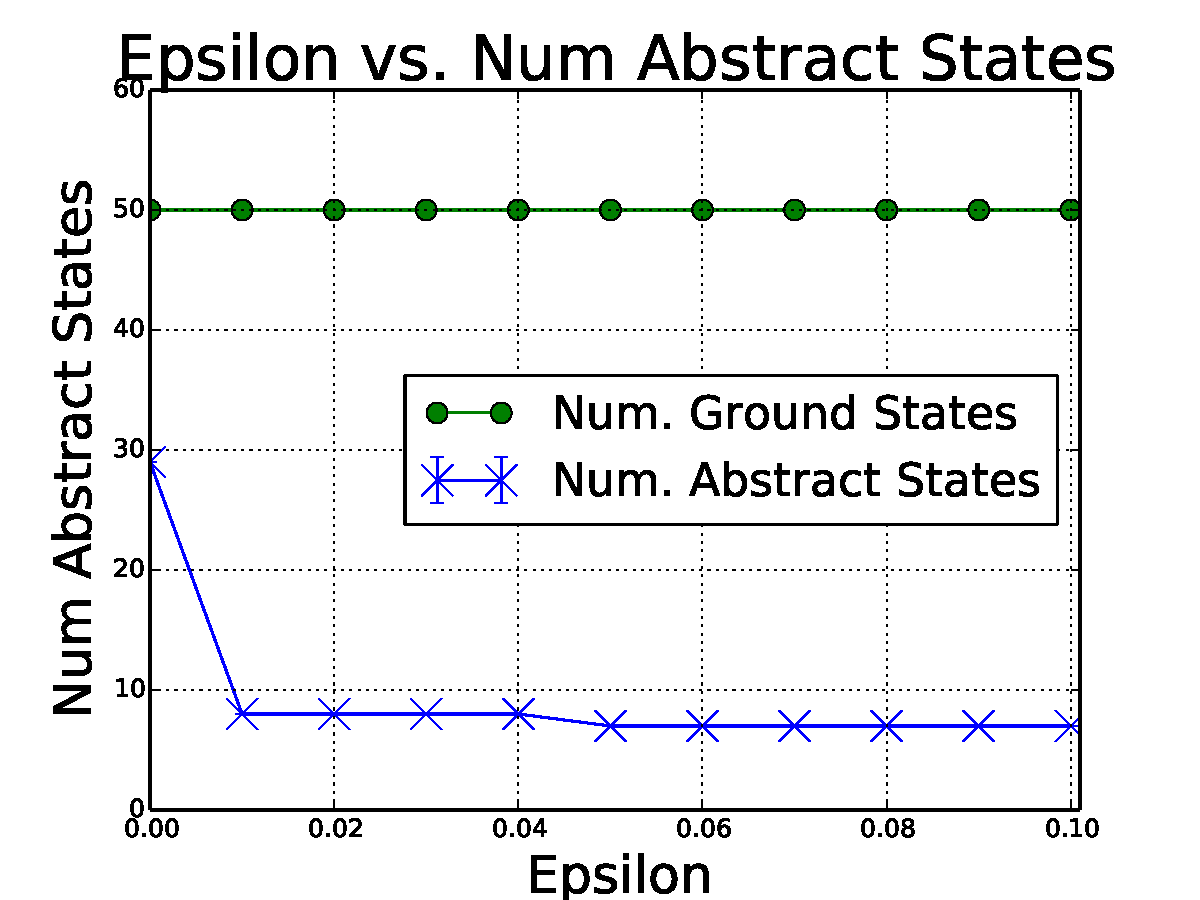
\includegraphics[width=0.46\columnwidth]{figures/nchain_epsilon_vs_num_abstract_states.pdf}
}
\subfigure[Minefield]{
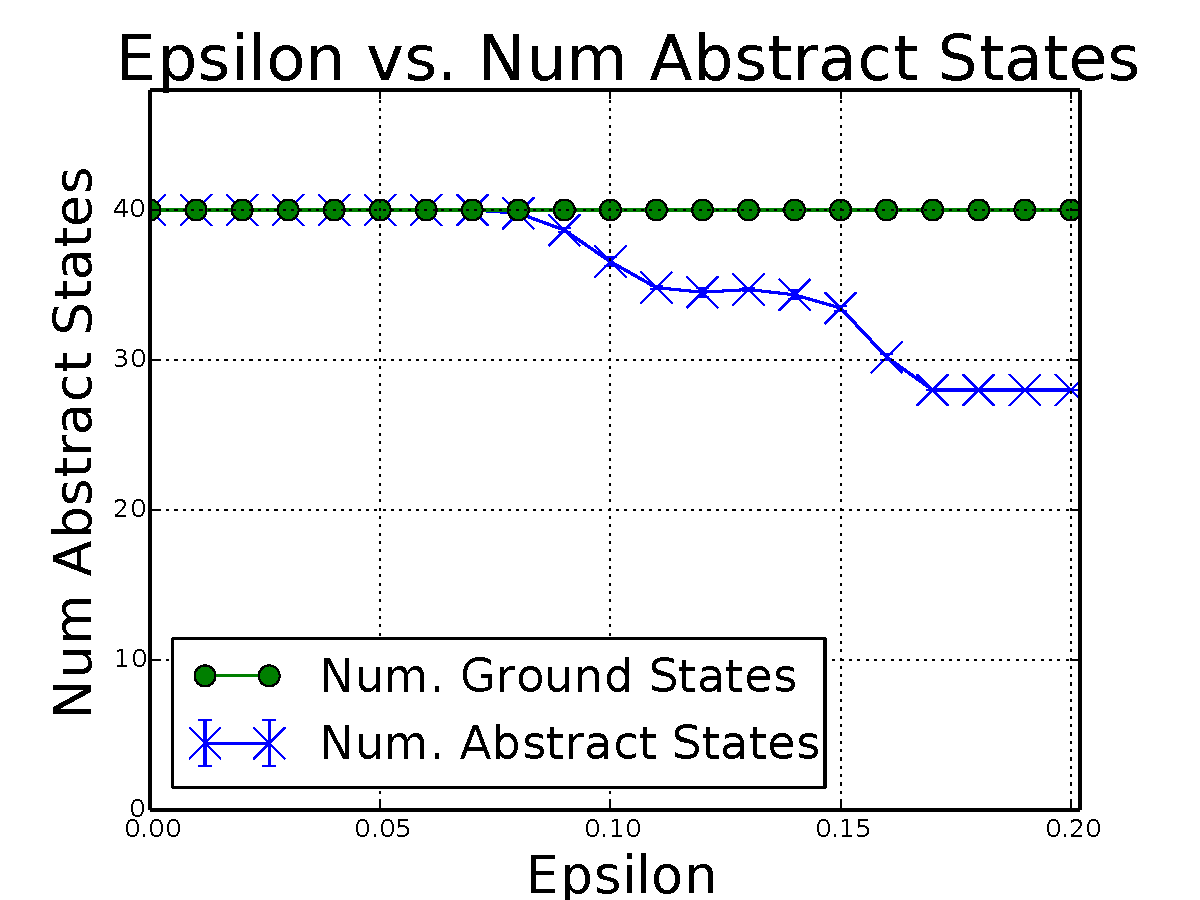
\includegraphics[width=0.46\columnwidth]{figures/minefield_epsilon_vs_num_abstract_states.pdf}
}
\subfigure[Taxi]{
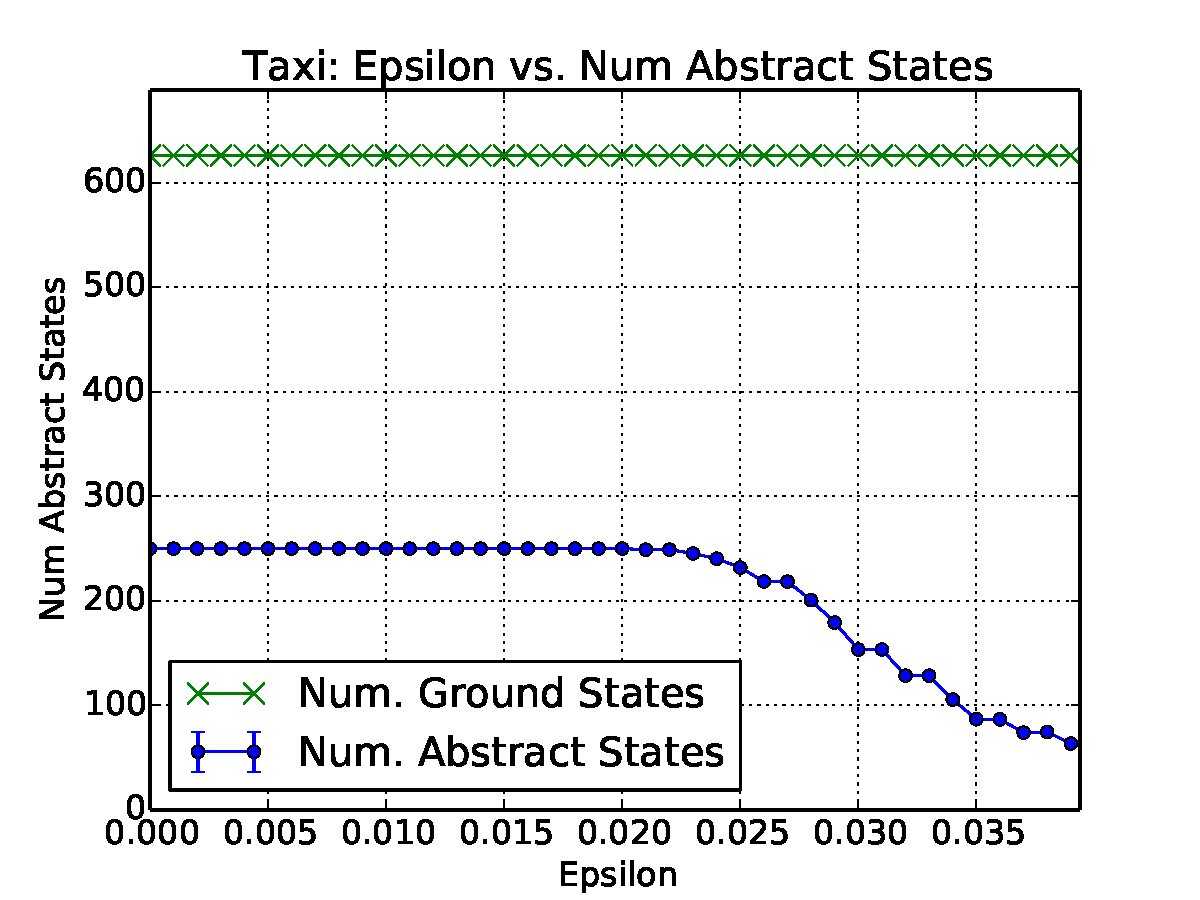
\includegraphics[width=0.46\columnwidth]{figures/taxi_epsilon_vs_num_abstract_states.pdf}
}
\subfigure[Random]{
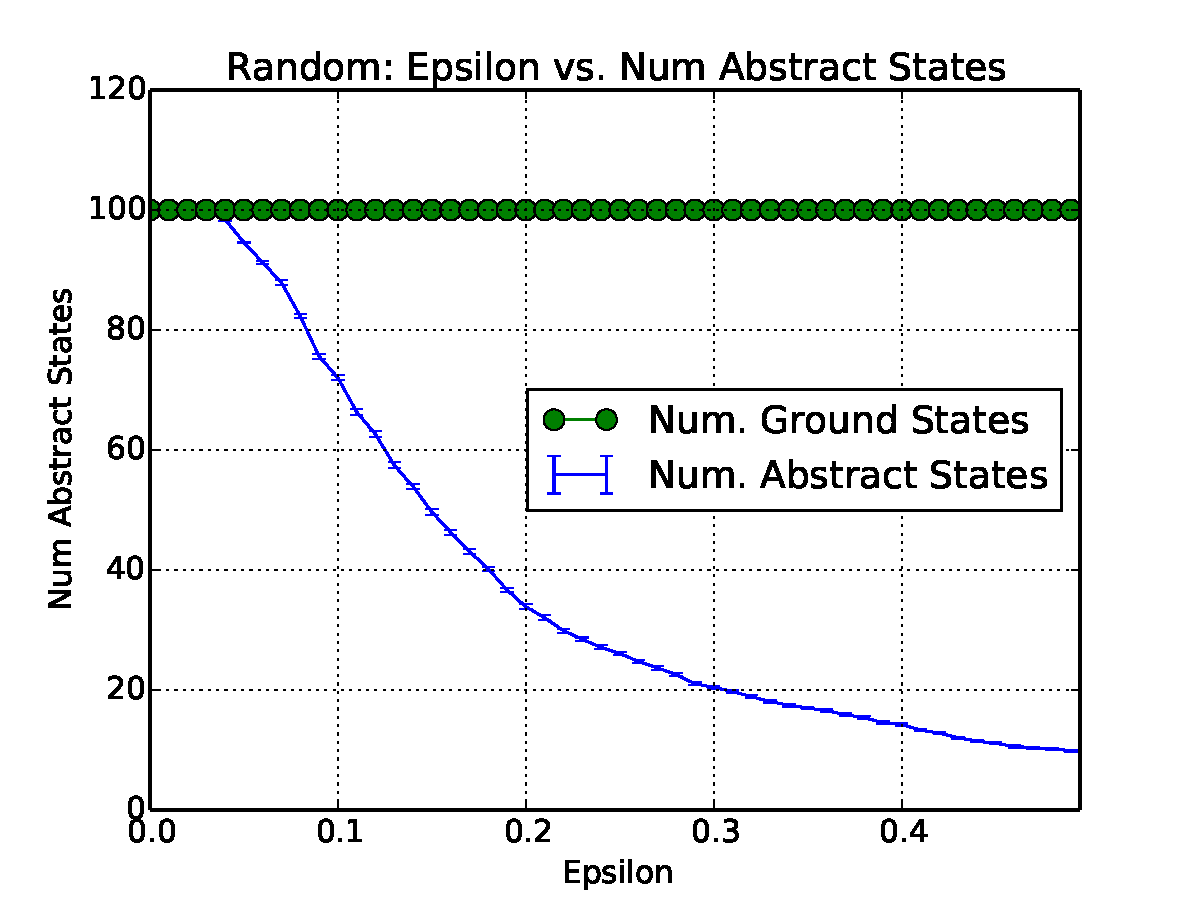
\includegraphics[width=0.46\columnwidth]{figures/random_epsilon_vs_num_abstract_states.pdf}
}

\subfigure[NChain]{
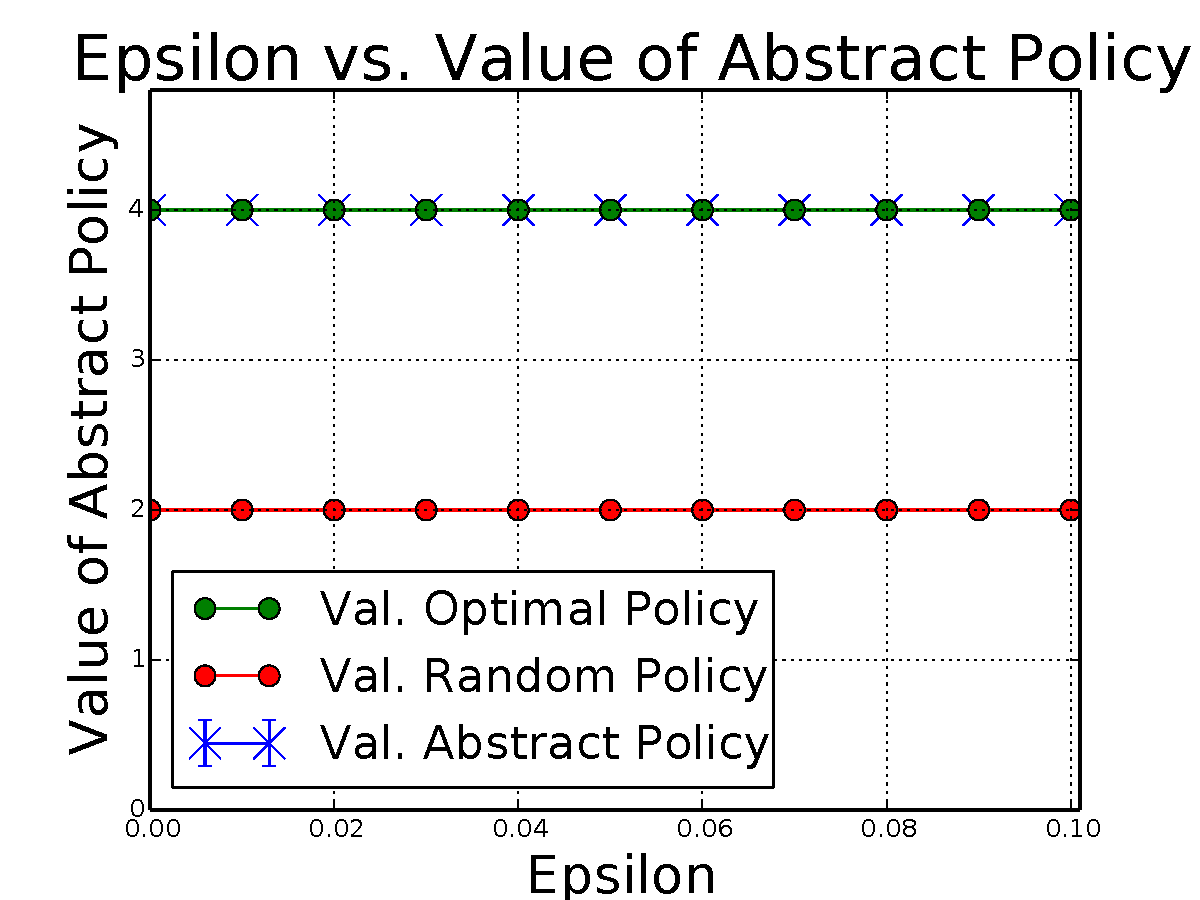
\includegraphics[width=0.46\columnwidth]{figures/nchain_epsilon_vs_value_of_abstract_policy.pdf}
}
\subfigure[Minefield]{
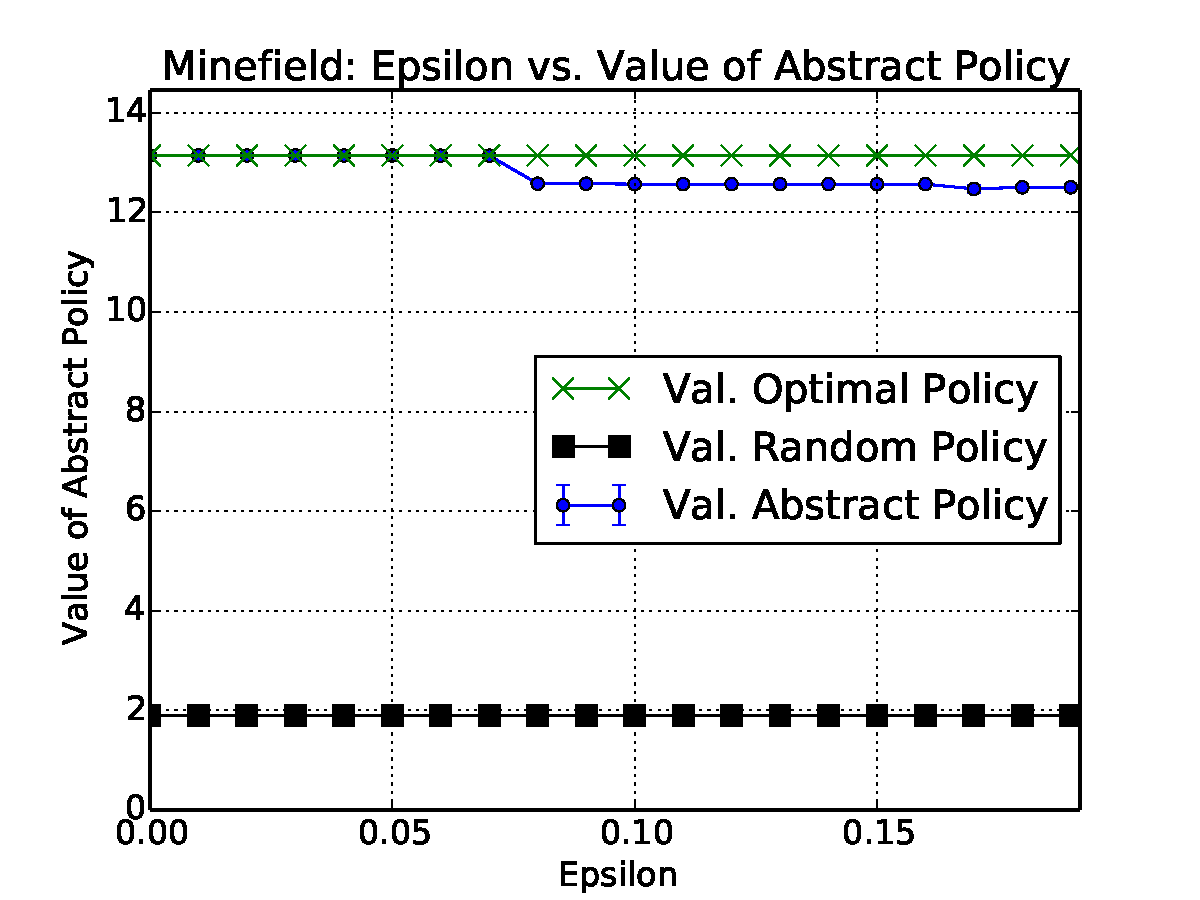
\includegraphics[width=0.46\columnwidth]{figures/minefield_epsilon_vs_value_of_abstract_policy.pdf}
}
\subfigure[Taxi]{
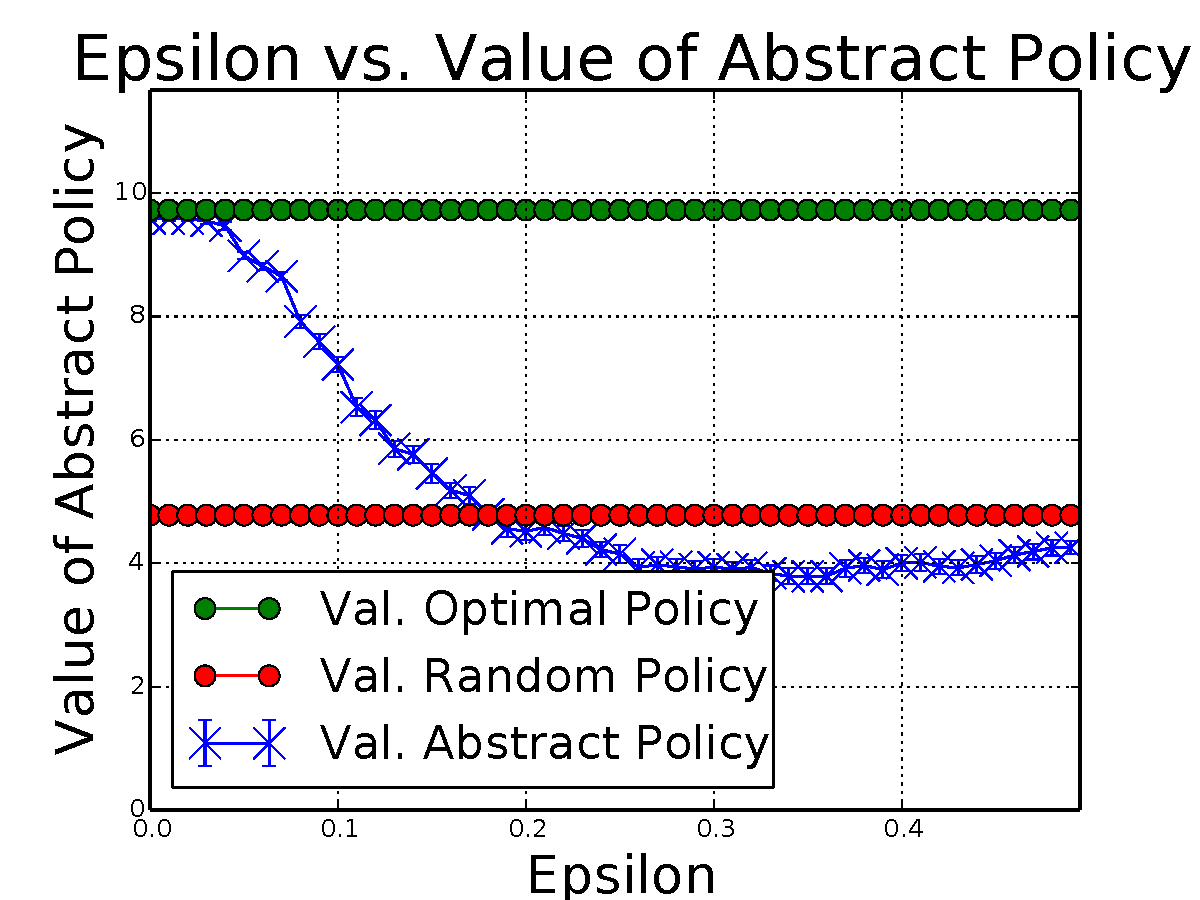
\includegraphics[width=0.46\columnwidth]{figures/taxi_epsilon_vs_value_of_abstract_policy.pdf}
}
\subfigure[Random]{
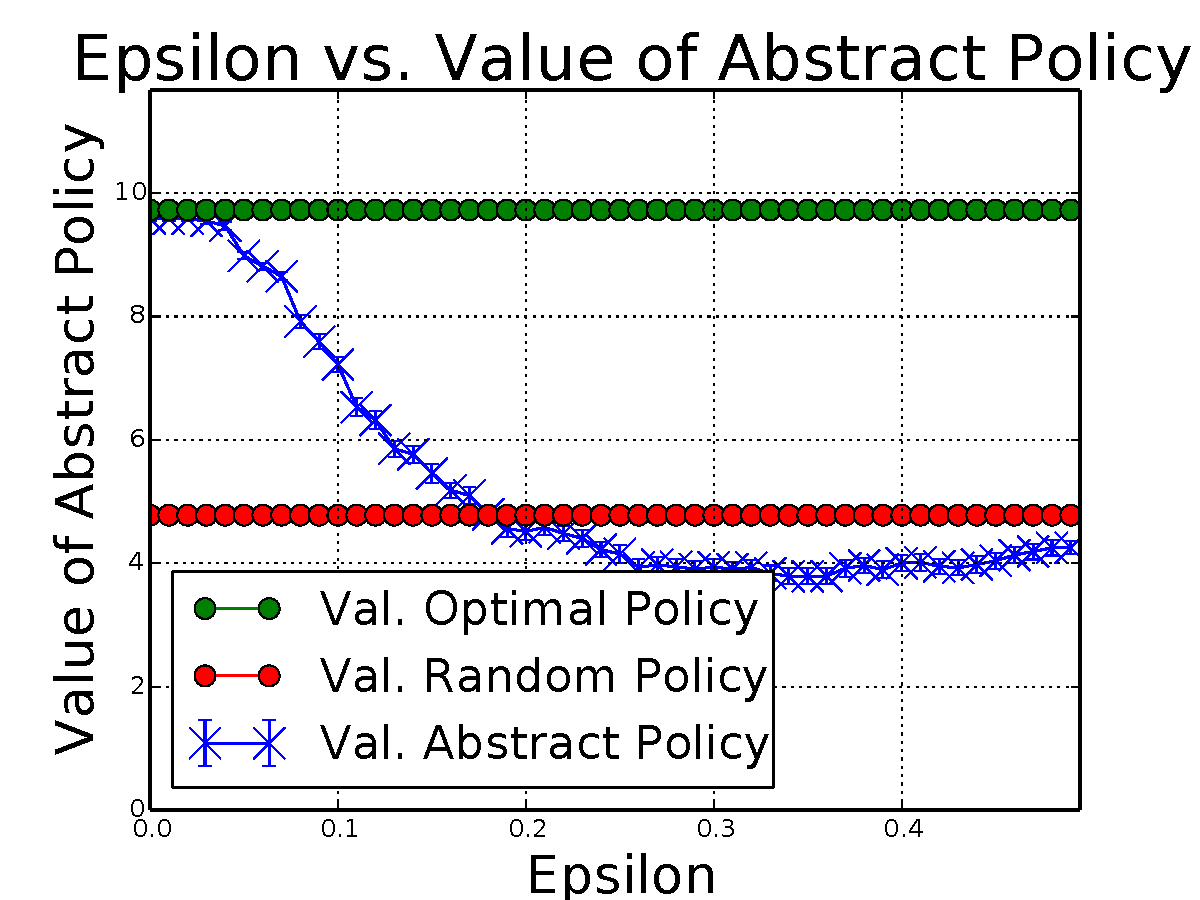
\includegraphics[width=0.46\columnwidth]{figures/random_epsilon_vs_value_of_abstract_policy.pdf}
}
\caption{$\varepsilon$ vs. Num States and $\varepsilon$ vs. Abstract Policy Value\label{fig:main_empirical_results1}}
\end{figure*} 

% Figure: Epsilon vs. #States and Epsilon vs Abstract Pol. For Taxi and Random.
%\begin{figure}
%\label{fig:main_empirical_results2}
%\centering
%\caption{$\varepsilon$ vs. Num States and $\varepsilon$ vs. Abstract Policy Value}
%\end{figure} 
